\documentclass{article}
\usepackage{graphicx}
\usepackage{amsmath,amssymb}
\title{基于“总量—等权”结构的洪水灾害数据分析与概率预测}
\author{}
\date{}
\begin{document}
\maketitle



\section*{摘要}

本文基于 104.9 万条洪水训练数据，用取证式分析揭示了一个被常规相关性排序掩盖的事实：20 个指标近似可交换，目标几乎是行总和 \(N\) 的线性函数，
\[
\hat y=0.00564676\,N-0.053355,\qquad R^2=0.8450,
\]
残差标准差仅 0.0201 且与所有指标无关。控制 \(N\) 后指标两两相关约为 \(-1/19\)，符合“把 \(N\) 个计数单元多项分配到 20 个指标”的机制；\(N\) 本身多峰。因此本题的核心是识别一个等权综合致灾指数，而不是寻找关键指标。

问题 1 用 Pearson/Spearman、互信息、置换重要性、留一 \(R^2\) 和自助法分析。20 个指标的单变量 \(r\) 仅在 \([0.1778,0.1902]\)，自助法 95\% 排名区间平均宽度 15.7（满量程 20）；四种重要性度量的排序甚至负相关（Pearson 与置换重要性的 Spearman 为 \(-0.40\)）。因此不存在稳健的关键指标。进一步的等权约束检验显示，严格等权虽被 104.9 万样本拒绝（\(p=1.2\times10^{-10}\)），但 \(\Delta R^2\) 仅 \(1.3\times10^{-5}\)、系数偏差 \(<1\%\)，实践上等价。

问题 2 按目标三分位分级，风险组目标均值为 0.4497/0.5046/0.5609；三组的所有指标同步平移，\(\eta^2\) 仅 0.0236–0.0271，KMeans 与风险分级的 ARI 仅 \(7.3\times10^{-5}\)。熵权/CRITIC 都接近等权；TOPSIS 与目标的 Spearman 为 0.8805，三级预警一致率 71.5\%；权重约 \(\pm10\%\) 扰动下 Spearman 仍达 0.969。

进一步，本文反演出生成模型（\(N\) 的 GMM、欠离散多项分配、Student-\(t\) 噪声），并用 DAG、偏相关与干预模拟说明：\(N\) 是唯一可观测驱动变量，给定 \(N\) 后指标与 \(y\) 条件独立（偏相关 \(|r|\le0.0041\)），保持 \(N\) 不变的再分配对 \(y\) 无影响。

问题 3 比较六类模型：OLS、Ridge 与等权指数的验证集 RMSE 均为 0.02011，已达噪声下限；HistGB 为 0.02116，随机森林为 0.03533。穷举 15504 个五指标组合，RMSE 均落在 \([0.04604,0.04651]\)，最优五指标也仅 \(R^2=0.1844\)。

问题 4 对 745305 条测试数据预测，均值 0.5045、标准差 0.0469，并按原格式写回 \texttt{submit.csv}。预测信号多峰（峰度 0.841，KS \(D=0.0714\)），观测值因噪声叠加才接近正态（峰度 \(-0.039\)，KS \(D=0.0285\)）。因此预测信号非正态，观测值仅近似正态。

本文不迎合“关键指标”的常规叙事，而是用可复现的证据链说明数据的等权—总量结构。


\noindent\textbf{关键词：} 洪水概率；等权综合指数；多项分配；TOPSIS；五指标穷举；非正态多峰分布

\newpage

\section{问题重述}

附件给出 104.9 万条洪水训练数据，包含 20 个指标得分与洪水发生概率；测试集 74.5 万条只含指标，需要预测概率并填入 \texttt{submit.csv}。题目要求：

\begin{enumerate}[label=\textbf{问题 \arabic*}：]
  \item 分析 20 个指标中哪些与洪水发生密切相关、哪些关系不大，解释原因并提出提前预防建议；
  \item 将洪水概率聚类为不同风险类别，分析高/中/低风险事件的指标特征；选取指标、计算权重，建立风险预警评价模型并做灵敏度分析；
  \item 基于问题 1 的指标分析建立洪水概率预测模型，验证准确性；进一步讨论仅用 5 个关键指标时如何调整改进；
  \item 用问题 2（题面笔误，应为问题 3）的模型预测 \texttt{test.csv} 全部事件，填入 \texttt{submit.csv}，绘制概率直方图与折线图，分析分布是否服从正态分布。
\end{enumerate}

\section{问题分析}

\subsection{总体判断}
本题表面上是标准的“相关性分析—聚类—回归—提交”数据挖掘题，但数据本身具有强烈的结构。若直接套用随机森林、XGBoost、SHAP 等流程，很容易得到“某几个指标最重要”的结论；然而本文的取证分析表明，这种结论并不可靠。因此本文先回答“数据是怎么长出来的”，再回答四个问题。

\subsection{四问的逻辑关系}
\begin{itemize}
  \item 问题 1 决定“指标是否可分”。若 20 个指标近似等权（权重差异 $<1\%$），则排序的实践意义很小；
  \item 问题 2 决定“风险是否有类型”。若风险组只是所有指标同步平移，则预警模型应使用综合指数而非指标组合；
  \item 问题 3 决定“预测模型的上限”。线性等权模型若已达到噪声下限，复杂模型就没有必要；
  \item 问题 4 决定“分布结论”。预测信号与观测值可能具有不同的分布形态，不能混为一谈。
\end{itemize}

\section{模型假设}

\begin{enumerate}
  \item 附件数据真实反映题目设定的洪水致灾背景；指标得分越高表示致灾背景越不利（该方向由数据中的正相关经验支持）。
  \item 测试集与训练集同分布。第 \ref{sec:eda} 节的 KS 检验支持这一假设（20 个指标的最大 KS 统计量仅 0.00202）。
  \item 指标得分是离散计数型变量，取值 $0$–$18$；本文不假设其服从正态分布。
  \item 目标值中的观测噪声与 20 个指标独立。第 \ref{sec:eda} 节验证残差与所有指标的相关系数绝对值小于 $10^{-15}$。
  \item 风险等级按目标值三分位划分；预警等级按 TOPSIS 得分三分位划分。两者独立定义，避免循环论证。
\end{enumerate}

\section{符号说明}

\begin{table}[H]
\centering
\caption{主要符号}
\begin{tabular}{cl}
\toprule
符号 & 含义 \\
\midrule
$x_{ij}$ & 第 $i$ 个事件第 $j$ 个指标的得分，$j=1,\dots,20$ \\
$N_i=\sum_{j=1}^{20}x_{ij}$ & 第 $i$ 个事件的行总和 \\
$y_i$ & 第 $i$ 个事件的洪水发生概率 \\
$\varepsilon_i$ & 观测噪声 \\
$r_j$ & 第 $j$ 个指标与目标的 Pearson 相关系数 \\
$w_j$ & 第 $j$ 个指标的综合权重 \\
$C_i$ & 第 $i$ 个事件的 TOPSIS 贴近度 \\
\bottomrule
\end{tabular}
\end{table}

\section{数据探索与生成机制}\label{sec:eda}

\subsection{数据概况}
训练集 1,048,575 行 $\times$ 22 列（id + 20 指标 + 目标），测试集 745,305 行 $\times$ 21 列。训练集与测试集的特征均无缺失；测试集的目标列按设计缺失。20 个指标均为 $0$–$18$ 的整数，均值约 4.92–4.96，标准差约 2.05–2.09。目标范围 $[0.285,0.725]$，均值 0.5045，标准差 0.0510，共 83 个离散取值（步长 0.005）。

\begin{table}[htbp]
\centering
\caption{数据规模与基本统计}
\label{tab:data}
\small
\begin{tabular}{lrr}
\toprule
项目 & 训练集 & 测试集 \\
\midrule
训练集 & 1,048,575 & 22 \\
测试集 & 745,305 & 22 \\
缺失值（特征） & 0 & 0 \\
目标均值 & 0.5045 & — \\
目标标准差 & 0.0510 & — \\
目标范围 & [0.285, 0.725] & — \\
指标范围 & [0, 18] & 同左 \\
指标均值范围 & [4.922, 4.956] & 同左 \\
\bottomrule
\end{tabular}
\end{table}




\subsection{指标可交换性与负相关}
20 个指标的均值极差仅占均值的 0.68\%，标准差极差仅占 2.02\%，可视为近似可交换。更值得注意的是，任意两个指标的相关系数全部为负，范围 $[-0.0167,-0.0056]$，均值 $-0.0104$。这与“20 个独立风险因子”的直觉相反。

进一步，把行总和 $N$ 控制在窄区间内（如 $95\le N<100$）再计算两两相关，平均值约为 $-0.0514$，非常接近多项分配的理论值
\[
-\frac{1}{20-1}=-\frac{1}{19}\approx -0.0526.
\]
这说明数据很可能按如下机制生成：先抽取一个行总和 $N_i$，再把 $N_i$ 个计数单元近似等概率地分配到 20 个指标。于是指标之间存在“总量守恒”造成的弱负相关，而不是真正的风险因子相关。

\begin{figure}[H]
\centering
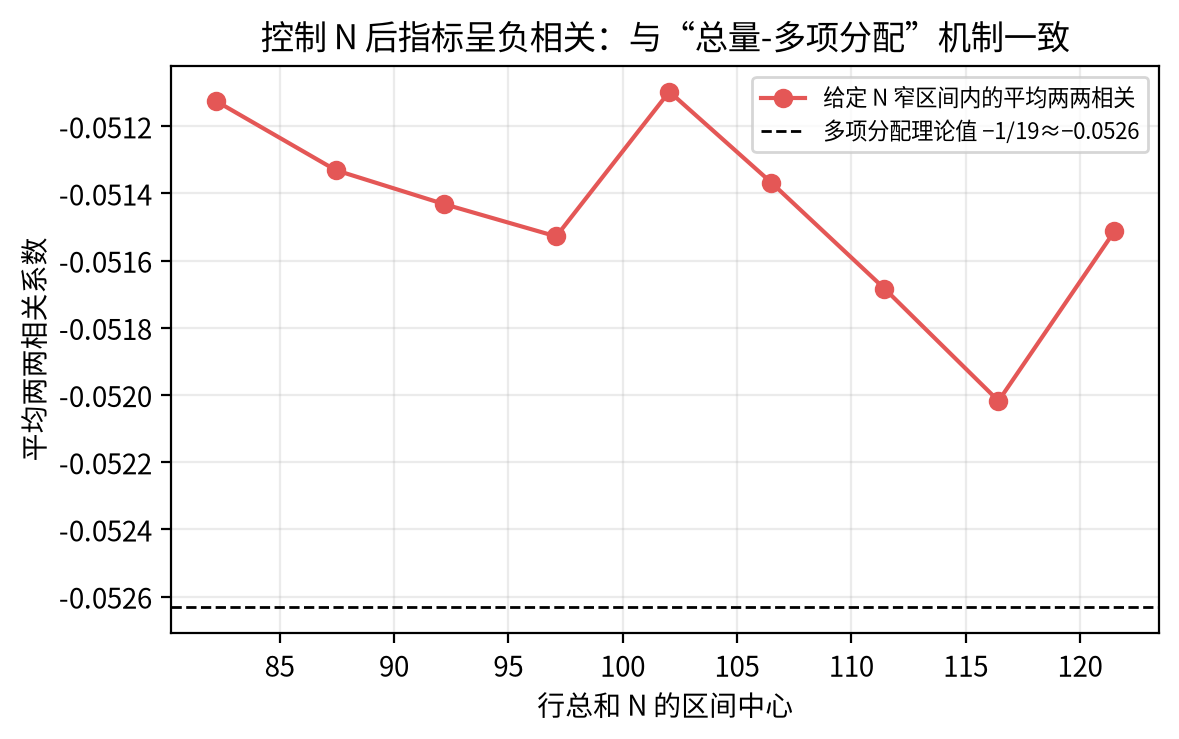
\includegraphics[width=0.95\textwidth]{../figures/fig_structure_corr.png}
\caption{控制行总和 $N$ 后，指标两两相关接近 $-1/19$}
\label{fig:structcorr}
\end{figure}

\subsection{行总和本身是多峰的}
行总和 $N$ 的均值为 98.79、标准差 8.31、范围 $[64,144]$。对 $N$ 拟合高斯混合模型，$k=4$ 已能捕捉主要峰（成分均值约 82.5、94.7、103.5、110.6，权重约 0.498、0.302、0.138、0.062）；第 6 节的生成模型取 $k=6$ 以更灵活地复现多峰。也就是说，$N$ 不是单峰正态，而是由多个“总量水平”混合而成。

\begin{figure}[H]
\centering
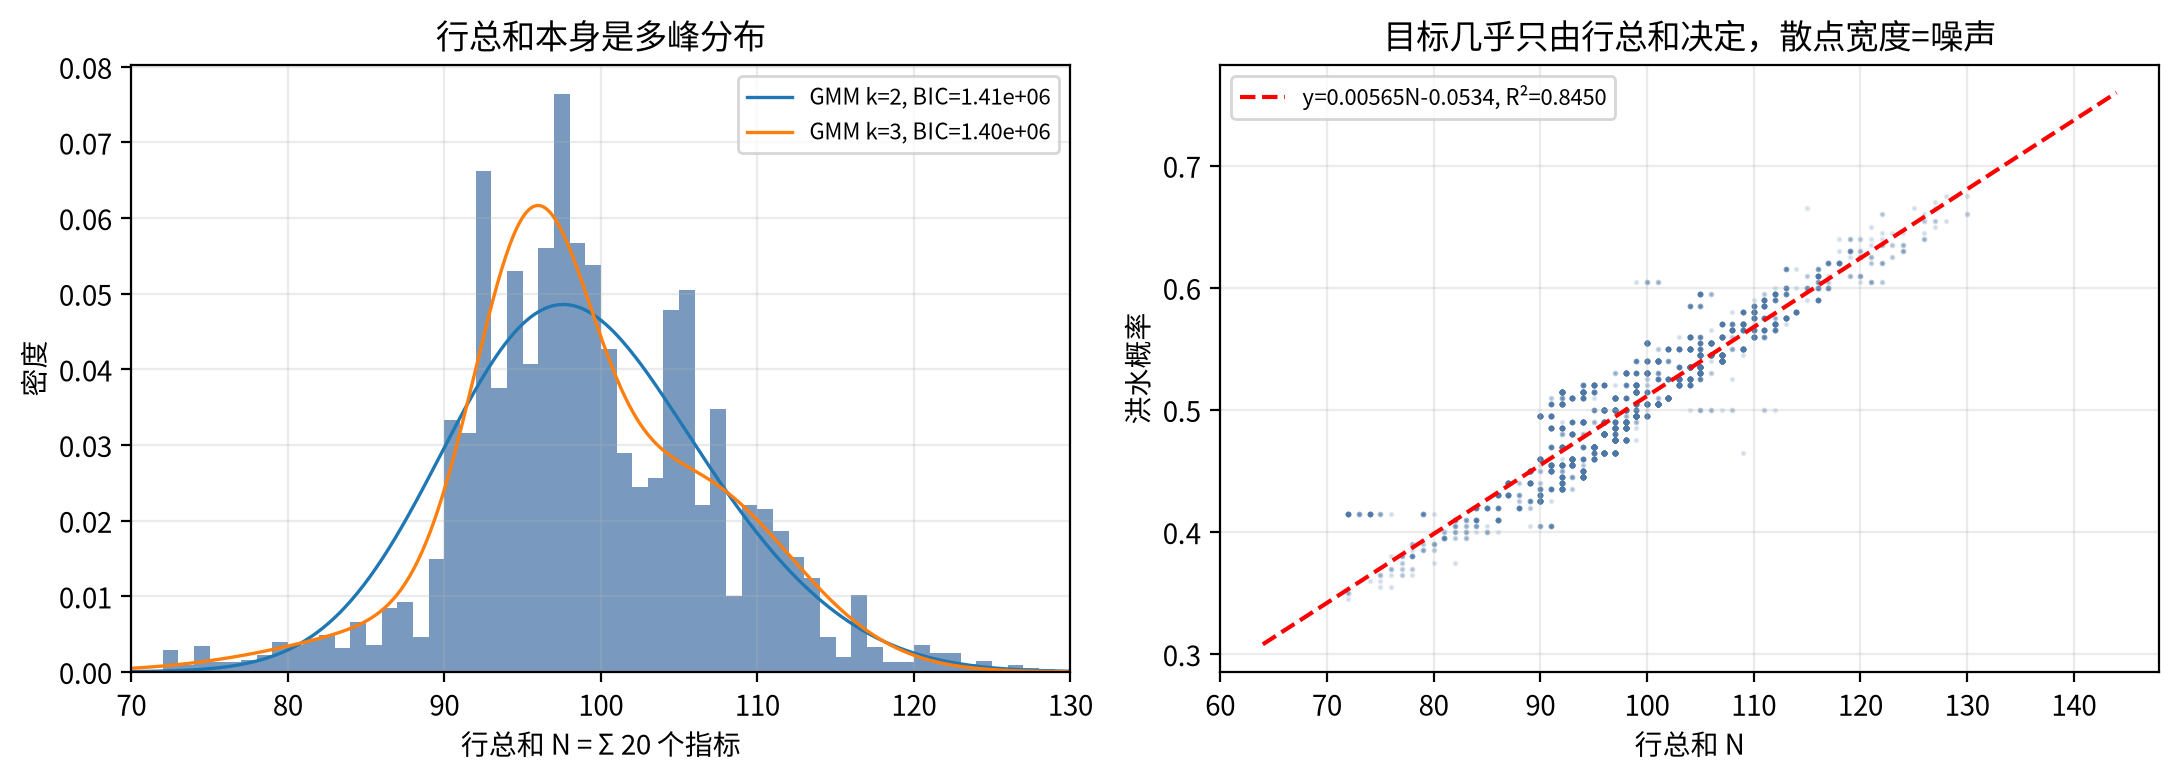
\includegraphics[width=0.95\textwidth]{../figures/fig_structure_rowsum.png}
\caption{左：行总和 $N$ 的多峰分布与 GMM 拟合；右：目标几乎只由 $N$ 决定}
\label{fig:structrowsum}
\end{figure}

\subsection{目标 = 行总和的线性函数 + 噪声}
以 $N$ 为唯一自变量对 $y$ 做线性回归，得到
\[
\hat y=0.00564676\,N-0.053355,\qquad R^2=0.8450,\qquad \text{RMSE}=0.02009.
\]
残差标准差 0.02009，占目标方差的 15.5\%；残差与 20 个指标的相关系数绝对值均小于 $10^{-15}$。这意味着：\textbf{给定行总和 $N$ 后，指标如何分配不再提供任何关于目标的信息}。目标只关心“总共有多少”，不关心“分在哪个指标上”。

\begin{table}[htbp]
\centering
\caption{数据结构与生成机制的关键证据}
\label{tab:structure}
\small
\begin{tabular}{lr}
\toprule
项目 & 数值 \\
\midrule
指标均值极差/均值 & 0.68\% \\
指标标准差极差/均值 & 2.02\% \\
两两相关均值 & -0.0104 \\
两两相关范围 & [-0.0167, -0.0056] \\
控制 N 后两两相关 & -0.0514 \\
多项分配理论值 $-1/19$ & -0.0526 \\
行总和 $N$ 均值 $\pm$ 标准差 & 98.79 $\pm$ 8.31 \\
行总和 N 范围 & [64, 144] \\
$y\approx aN+b$ 的 $R^2$ & 0.8450 \\
信号标准差 / 噪声标准差 & 0.0469 / 0.0201 \\
噪声占方差比例 & 15.50\% \\
\bottomrule
\end{tabular}
\end{table}


\subsection{对四问的启示}
上述结构直接决定了后文的建模路线：
\begin{itemize}
  \item 问题 1：单个指标与目标的相关只是“它占总量的一份”，不存在独立的关键指标；
  \item 问题 2：风险等级由 $N$ 决定，风险组的所有指标会同步平移，不应期待“组合型”画像；
  \item 问题 3：最优预测器就是 $N$ 的线性函数，即等权指数；复杂模型不会超过噪声下限；
  \item 问题 4：预测信号 $0.00564676N-0.053355$ 继承 $N$ 的多峰性；观测值 $y$ 因叠加噪声才变平滑。
\end{itemize}
在进入四问之前，第 6、7 节先把“数据怎么生成、\(N\) 为什么是混杂变量”说清楚：第 6 节用生成式反演还原数据生成过程，第 7 节用 DAG、条件独立与干预模拟做因果敏感性分析；四问是同一机制的四个观测角度。

\section{生成式逆向建模}

\subsection{从“工作模型”到可估计的生成模型}
第 \ref{sec:eda} 节只给出了条件均值层面的工作模型。为了把“数据是怎么长出来的”还原到可模拟、可检验的程度，本文把它写成显式的生成模型：
\[
\begin{aligned}
N_i &\sim \mathrm{GMM}(k=6),\\
(x_{i1},\dots,x_{i20})\mid N_i &\sim \mathrm{Underdispersed\ Multinomial}(N_i;p_1,\dots,p_{20};\phi),\\
y_i &= aN_i+b+\varepsilon_i,\qquad \varepsilon_i\sim \mathrm{Student\text{-}}t(\nu,\mu_\varepsilon,\sigma_\varepsilon).
\end{aligned}
\]
其中第二行表示“多项分配核心 + 均摊余量”：先按 \(p_j\) 随机分配 \(\phi N\) 个计数单元，再把剩余 \((1-\phi)N\) 个单元较均匀地摊到 20 个指标上。\(\phi<1\) 对应数据中“比标准多项分布更均匀”的欠离散现象。

参数全部由极大似然/矩估计得到：
\begin{itemize}
  \item \(p_j=\sum_i x_{ij}/\sum_i N_i\)，估计结果为 \(p_j\in[0.0498,0.0502]\)，与 \(1/20\) 几乎完全一致；
  \item 欠离散系数 \(\phi=\mathrm{Var}(x_j-Np_j)/\mathbb{E}[Np_j(1-p_j)]=0.8805\)；
  \item \(N\) 的 GMM 在 \(k=6\) 后 BIC 改善趋缓（\(k=6\to8\) 的相对改善不足 0.15\%），取 \(k=6\)；
  \item 噪声用 Student-\(t\) 拟合，\(\nu=8.22\)、\(\sigma_\varepsilon=0.0175\)；相比高斯，NLL 从 \(-2.4948\) 降到 \(-2.5033\)，说明残差有轻度重尾。
\end{itemize}

\begin{table}[htbp]
\centering
\caption{生成模型的参数估计（反演结果）}
\label{tab:generative}
\small
\begin{tabular}{llr}
\toprule
模块 & 参数 & 估计值 \\
\midrule
$N$ 分布 & GMM 成分数 $k$ & 6 \\
$N$ 分布 & 成分均值范围 & [82.67, 117.75] \\
$N$ 分布 & 成分标准差范围 & [1.78, 5.47] \\
分配 & $p_j$ 范围 & [0.0498, 0.0502] \\
分配 & 欠离散系数 $\phi$ & 0.8805 \\
噪声 & 高斯 $\sigma$ & 0.0201 \\
噪声 & Student-$t$ $df$ / scale & 8.22 / 0.0175 \\
目标 & $a$ / $b$ & 0.005647 / -0.0534 \\
目标 & $R^2$ / RMSE & 0.8450 / 0.0201 \\
潜在机制 & oracle / 可部署 RMSE & 0.0115 / 0.0202 \\
潜在机制 & 可由 $x$ 识别（AUC） & 0.535 \\
\bottomrule
\end{tabular}
\par\vspace{2pt}\footnotesize $N$ 的 GMM 在 $k=6$ 后 BIC 改善趋缓；$\phi<1$ 表示分配比多项分布更均匀。
\end{table}


\subsection{模拟复现（后验预测检验）}
用估计出的生成模型独立模拟 20 万条数据，并与真实数据做后验预测检验（PPC）。结果见表 4 与图 3：行总和均值/标准差、目标均值/标准差、指标两两相关、控制 \(N\) 后相关、\(y\sim N\) 的 \(R^2\) 都能复现；唯一偏差是指标标准差略高（2.131 vs 2.075，约 \(+2.7\%\)），说明“均摊余量”的随机化仍带来少量额外方差。这个偏差不影响机制结论，但提示生成模型在方差层面还可以继续细化。

\begin{figure}[H]
\centering
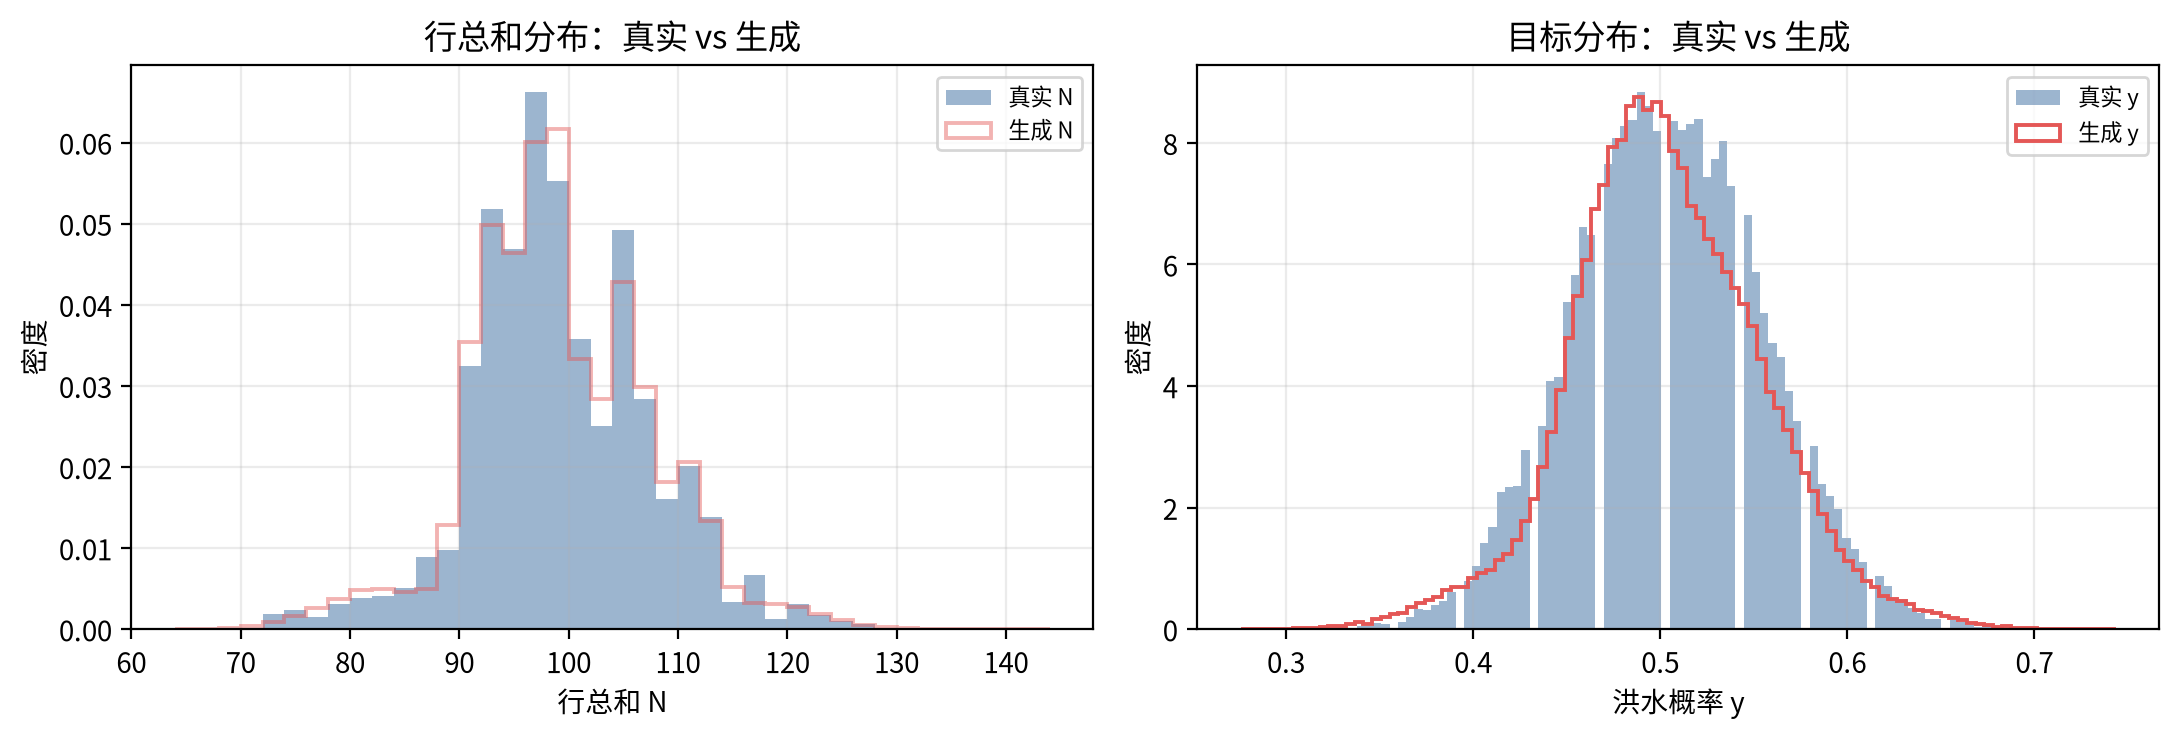
\includegraphics[width=0.95\textwidth]{../figures/fig_generative_ppc.png}
\caption{生成模型对行总和与目标分布的复现}
\label{fig:genppc}
\end{figure}

\subsection{生成模型预测 vs OLS}
由于 \(N_i=\sum_j x_{ij}\) 在预测时完全已知，生成模型的条件均值就是
\[
\mathbb{E}[y\mid x]=\mathbb{E}[y\mid N]=aN+b,
\]
与 OLS/等权指数\textbf{完全相同}。因此二者的点预测 RMSE 都是 0.02011——生成模型不会、也不应该提高点精度。生成模型的价值在于给出完整的预测分布，而不是只给一个点。

表 5 比较了三种噪声假设的预测分布。Student-\(t\) 的 NLL/CRPS 略优于高斯（约 0.3\%–0.5\%），95\% 覆盖率与高斯相当；经验残差分布的 CRPS 最好，但直接使用训练集分位数会导致验证集覆盖率略低（93.5\%），实际使用时应做分位数校准或共形预测。

\begin{table}[htbp]
\centering
\caption{生成模型与 OLS 的预测分布对比}
\label{tab:generativepred}
\small
\begin{tabular}{lrrrr}
\toprule
噪声模型 & NLL & CRPS & 95\% 覆盖率 & 区间宽度 \\
\midrule
高斯 & -2.4948 & 0.01123 & 94.71\% & 0.07865 \\
Student-t & -2.5033 & 0.01118 & 93.97\% & 0.08043 \\
经验残差 & — & 0.01107 & 93.52\% & 0.07429 \\
\bottomrule
\end{tabular}
\par\vspace{2pt}\footnotesize 点预测完全相同（RMSE=0.02011）；生成模型的差异只在预测分布。
\end{table}




\subsection{潜在机制异质性：一个不可部署的上界}
残差诊断还发现一个更强的结构：若允许两个潜在的线性机制
\[
y_i=a_{R_i}N_i+b_{R_i}+\varepsilon_i,\qquad R_i\in\{1,2\},
\]
并用 \(y\) 的后验责任去拟合，则验证集 RMSE 可降到 0.0115（约为单机制的一半）。但这只是\textbf{oracle 上界}：在真实预测时 \(R_i\) 不可观测。若只用 \(N\) 做门控，验证集 RMSE 为 0.02017，反而略差于单机制 OLS；若用 20 个指标去预测 \(R_i\)，AUC 仅 0.535。也就是说，潜在机制既不能由 \(N\) 识别，也不能由指标识别，只能作为不可观测异质性。因此本文仍以单机制等权模型作为可部署预测器，把双机制结果作为“数据中还存在未解释结构”的诊断。

\section{因果敏感性分析}

\subsection{DAG 与可识别性}
本文没有干预实验，不能做严格因果推断；但可以在明确 DAG 假设下做\textbf{因果敏感性分析}。生成模型对应的因果图是：
\[
N\longrightarrow x_j\ (j=1,\dots,20),\qquad N\longrightarrow y,\qquad R\longrightarrow y,
\]
其中 \(R\) 是潜在机制，且经验上 \(R\) 与 \(x\) 近似独立（AUC=0.535）。在这个 DAG 中，\(N\) 是 \(x_j\) 与 \(y\) 的\textbf{混杂变量}：\(x_j\) 对 \(y\) 的边际相关，来自它和 \(y\) 共享同一个 \(N\)；给定 \(N\) 后，\(x_j\) 与 \(y\) 应该条件独立。

\begin{figure}[H]
\centering
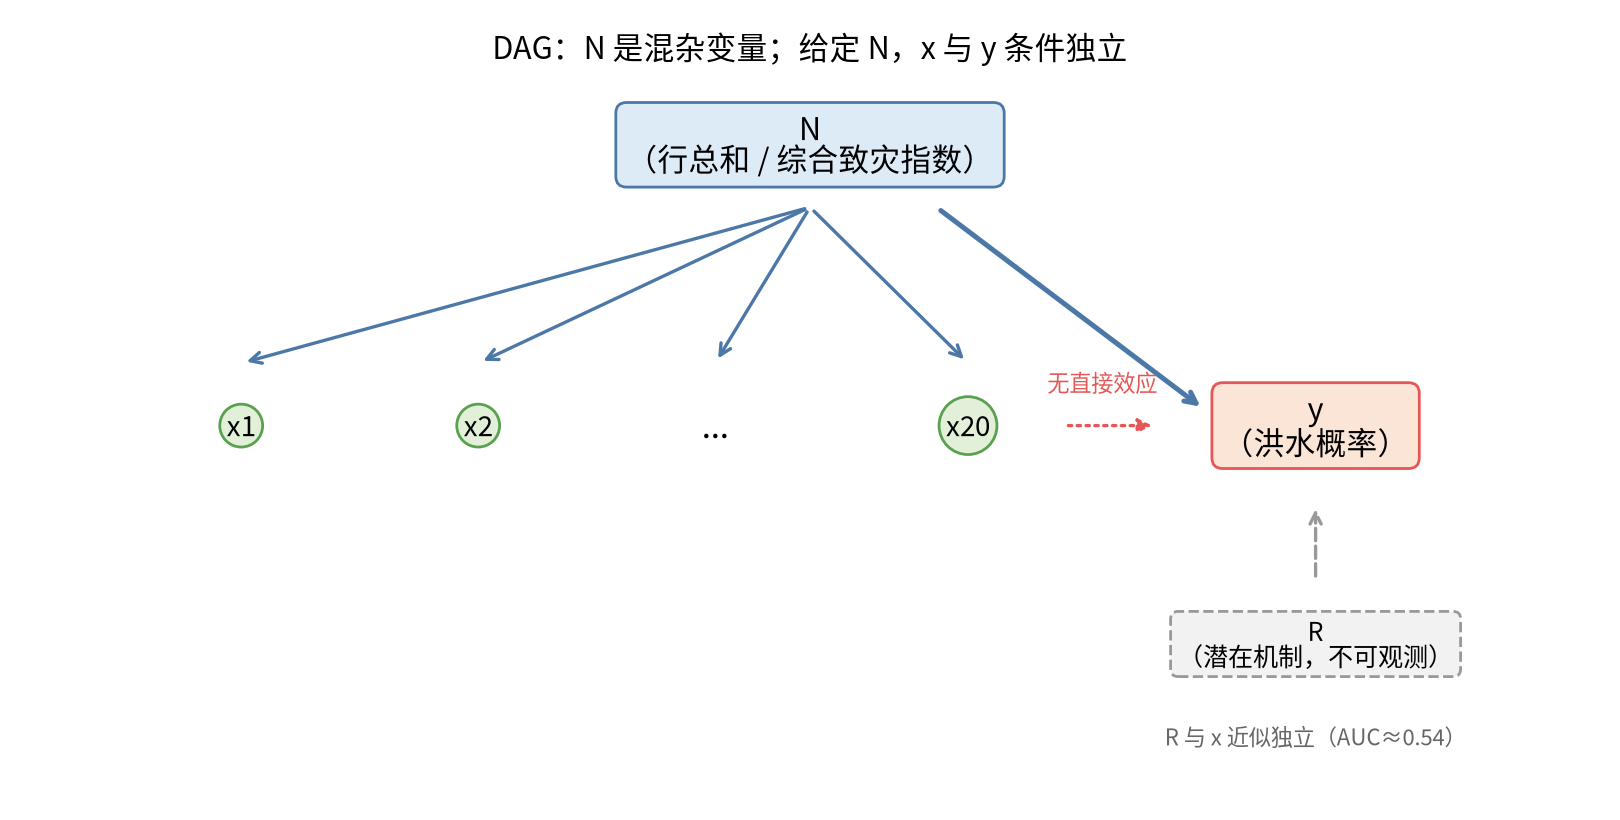
\includegraphics[width=0.82\textwidth]{../figures/fig_causal_dag.png}
\caption{因果假设：\(N\) 是混杂变量，指标没有直接指向 \(y\) 的边}
\label{fig:causaldag}
\end{figure}

\subsection{条件独立检验}
对每个指标计算边际相关与偏相关：
\[
r_j^{\text{marg}}=\mathrm{Corr}(x_j,y),\qquad
r_j^{\text{partial}}=\mathrm{Corr}\big(x_j-\mathbb{E}[x_j|N],\ y-\mathbb{E}[y|N]\big).
\]
结果见表 6：边际相关全部在 \(0.178\)–\(0.190\)，但给定 \(N\) 后偏相关全部落在 \([-0.0041,0.0039]\)，偏 \(R^2\) 最大仅 \(0.0017\%\)。部分偏相关的 \(p\) 值因 \(n=10^6\) 而“显著”，但效应量比噪声低两个数量级，应看效应量而不是 \(p\) 值。

\begin{table}[htbp]
\centering
\caption{因果敏感性：边际相关与条件独立检验汇总}
\label{tab:causalsummary}
\small
\begin{tabular}{lr}
\toprule
统计量 & 数值 \\
\midrule
边际 $r(x_j,y)$ 范围 & [0.1778, 0.1902] \\
偏相关 $r(x_j,y|N)$ 范围 & [-0.0041, 0.0039] \\
偏 $R^2$ 最大 & 0.00167\% \\
控制 $N$ 后指标间平均相关 & -0.0481 \\
\bottomrule
\end{tabular}
\par\vspace{2pt}\footnotesize 偏相关为给定 $N$ 后的条件相关；偏 $R^2$ 为在 $y\sim N$ 基础上加入 $x_j$ 的增量。
\end{table}




\subsection{干预模拟}
在拟合好的生成模型上做“模型内干预”，结果见表 7：
\begin{itemize}
  \item 保持 \(N\) 不变、把 1 分从一个指标转移到另一个指标：\(\Delta y=0\)；
  \item 给任意一个指标加 1 分（\(N\to N+1\)）：\(\Delta y=\beta=0.00565\)；
  \item 20 个指标各加 1 分（\(N\to N+20\)）：\(\Delta y=20\beta=0.1129\)；
  \item 潜在机制从 1 切到 2（同一 \(N=99\)）：\(\Delta y\approx0.028\)，但该机制不可观测、不可干预，只能作为敏感性上界。
\end{itemize}
因此，\textbf{唯一可操作的因果杠杆是行总和 \(N\)，而不是某个单项指标}。这与第 \ref{sec:eda} 节的“总量—等权”结构完全一致。

\begin{table}[htbp]
\centering
\caption{干预模拟：只有改变 $N$ 才会改变 $y$}
\label{tab:intervention}
\small
\begin{tabular}{p{0.28\linewidth}p{0.20\linewidth}rp{0.30\linewidth}}
\toprule
干预 & 操作 & $\Delta y$ & 解释 \\
\midrule
保持 N 不变，重新分配 20 个指标 & x\_j 之间转移 1 分 & 0.0000 & 给定 N，y 与分配无关 \\
N 增加 1（随机给某个指标 +1） & N -> N+1 & 0.0056 & 总量效应 $\beta$ \\
20 个指标各 +1 & N -> N+20 & 0.1129 & 总量效应 ×20 \\
把 1 分从指标 j 转到指标 k & N 不变 & 0.0000 & 纯分配干预，无直接效应 \\
潜在机制从 1 切到 2（同一 N） & R: 1->2 & 0.0281 & 不可观测、不可干预，仅作敏感性 \\
\bottomrule
\end{tabular}
\par\vspace{2pt}\footnotesize 潜在机制切换取 $N=99$；该机制不可观测、不可干预，只用于敏感性分析。
\end{table}


\subsection{效应异质性与边界}
潜在机制使 \(N\to y\) 的斜率在 \([0.00438,0.00614]\) 之间变化，均值为 \(0.00565\)；这是“同一 \(N\) 下仍存在未观测异质性”的体现。由于 \(R\) 与 \(x\) 近似独立（AUC=0.535），没有证据表明某个指标能替代 \(N\) 或绕过 \(N\) 影响 \(y\)。因此本文的因果结论应表述为：
\begin{quote}
在“\(N\) 是混杂变量、指标无直接边”的 DAG 假设下，数据与“单项指标无直接因果效应”一致；可操作的只有总量 \(N\)。这不是干预实验的因果证明，而是对“相关性全部由 \(N\) 解释”这一机制的敏感性分析。
\end{quote}

\section{问题 1：指标关联分析}

\subsection{方法}
对每个指标 $j$ 计算：
\begin{enumerate}
  \item Pearson 相关 $r_j$ 与 Spearman 秩相关，并给出 Fisher $z$ 的 95\% 置信区间；
  \item 互信息（把指标视为离散变量，抽样 6 万条估计）；
  \item 置换重要性：在 20 万条验证样本上随机打乱第 $j$ 个指标，记录 RMSE 增量，重复 10 次；
  \item 留一 $R^2$：从 20 维线性模型中删去第 $j$ 个指标，记录 $R^2$ 下降量；
  \item 自助法排名：重复 200 次、每次抽 5 万条，计算 20 个指标的 $r$ 排名，得到每个指标的 95\% 排名区间。
\end{enumerate}

\subsection{结果}
20 个指标的单变量相关全部落在 $[0.1778,0.1902]$，对应单变量 $R^2$ 仅 3.16\%–3.62\%；Spearman 秩相关在 $[0.1703,0.1814]$。从数值上看，排名第一与排名最后的指标差距不到 0.013，实际可忽略。




自助法结果非常直接：每个指标的 95\% 排名区间平均宽度为 15.7（满量程 20）。例如排名均值最靠前的“基础设施恶化”也只有 4.47，其 95\% 区间覆盖第 1–13 名；排名最后的“海岸脆弱性”区间覆盖第 6–20 名。也就是说，换一批样本，排名会大幅重排。

更关键的是，不同重要性度量给出的排序并不一致：
\begin{itemize}
  \item Pearson 与互信息的 Spearman 仅 0.322；
  \item Pearson 与置换重要性的 Spearman 为 $-0.400$（负相关）；
  \item Pearson 与留一 $R^2$ 的 Spearman 为 $-0.358$；
  \item 置换重要性与留一 $R^2$ 的 Spearman 为 0.946（二者都是条件重要性，较一致）。
\end{itemize}
边际相关与条件重要性甚至反向，这是因为指标之间存在“总量守恒”的负相关：某个指标边际上占总量的一份，条件上却要与其他指标竞争总量。因此，\textbf{“哪个指标最重要”没有唯一答案，取决于你用哪种度量}。

\subsection{等权约束检验与 Shapley 分解}

相关性排序只能说明“差异很小”，但不能回答“差异是否可以忽略”。为此把 20 个斜率约束为相等，即 \(y=a+\beta\sum_j x_j+\varepsilon\)，再与无约束 OLS 做嵌套比较。

\begin{table}[htbp]
\centering
\caption{等权约束与无约束 OLS 的对比}
\label{tab:p1equal}
\small
\begin{tabular}{lrrrr}
\toprule
模型 & $R^2$ & RMSE & 参数个数 & 系数极差/均值 \\
\midrule
无约束 OLS（20 指标） & 0.84502 & 0.020090 & 21 & 1.33\% \\
等权约束（行总和 $N$） & 0.84500 & 0.020091 & 2 & 0.00\% \\
\bottomrule
\end{tabular}
\par\vspace{2pt}\footnotesize 嵌套 F 检验 $F(19,1048554)=4.58$，$p=1.2\times10^{-10}$；$\Delta R^2=1.3\times10^{-5}$。随机分半的系数排序 Spearman $\rho=0.756$；Shapley $R^2$ 每项 0.0409–0.0434，极差仅 5.9\% 于均值。
\end{table}




结果有三层：
\begin{enumerate}
  \item \textbf{统计上显著，实践上可忽略}：\(F(19,1048554)=4.58\)，\(p=1.2\times10^{-10}\)，严格等权被拒绝；但 \(R^2\) 只下降 \(1.3\times10^{-5}\)，RMSE 只差 \(8.3\times10^{-7}\)，20 个系数与等权斜率的相对偏差最大仅 0.67\%（95\% CI 上限 1.00\%）。这是大样本下“显著 $\neq$ 重要”的典型例子。
  \item \textbf{排序部分可复现，但幅度极小}：随机分半后两半系数排序的 Spearman 为 0.756，前五名重合 4/5，说明并非纯噪声；然而所有差异都在 1\% 以内，不足以支撑“重点监测某几个指标”的政策结论。
  \item \textbf{重要性度量不一致}：Shapley \(R^2\) 每项在 0.0409–0.0434 之间，极差仅占均值 5.9\%；它与留一 \(R^2\) 排名的 Spearman 仅 0.06，与单变量 \(R^2\) 的排序为 0.88。指标标准差从 2.052 到 2.094（相差 2.0\%），而 Shapley 贡献对 \(\beta_j^2\mathrm{Var}(x_j)\) 敏感，说明这点差异主要来自指标方差，而不是权重。
\end{enumerate}

因此，问题 1 的准确表述是“20 个指标近似等权、权重差异 $<1\%$”：既不是“完全等权”，也不是“存在关键指标”。相关性排序可以报告，但只能作为方向性参考。

\subsection{结论与预防建议}
问题 1 的正确答案不是列出一个“关键指标清单”，而是：
\begin{enumerate}
  \item 20 个指标近似等权：严格等权虽被大样本拒绝，但权重差异 $<1\%$、$\Delta R^2=1.3\times10^{-5}$，不存在实践上可辨识的强/弱指标；
  \item 洪水风险是一个等权综合致灾指数，任何单指标监测都会丢失大部分信息；
  \item 预防措施应“多维度协同”：改善排水与河流管理、提升大坝质量与基础设施、控制城市化与森林砍伐、加强季风与气候变化监测；
  \item 若资源有限，可按“治理成本/可操作性”排序，而不是按相关性排序；相关性差异不足 $1\%$，不能作为优先级依据；
  \item 建议建立综合致灾指数（见问题 2 的 TOPSIS），用总分做预警，用分项做诊断。
\end{enumerate}

\section{问题 2：风险分级、赋权与 TOPSIS 预警}

\subsection{风险分级与画像}
按目标三分位划分低/中/高风险，阈值约为 0.480 与 0.525，三组样本量分别为 357,693、344,729、346,153，目标均值分别为 0.4497、0.5046、0.5609。

对每个指标计算组均值与标准化差 $(\bar x_{g,j}-\bar x_j)/s_j$。结果显示：三个风险组的所有指标都同步平移，低风险组约 $-0.23\sigma$，高风险组约 $+0.23\sigma$，没有任何“某几个指标特别突出”的结构。单因素方差分析的 $\eta^2$ 仅为 0.0236–0.0271，即风险等级只能解释每个指标约 2.5\% 的方差。

\begin{figure}[H]
\centering
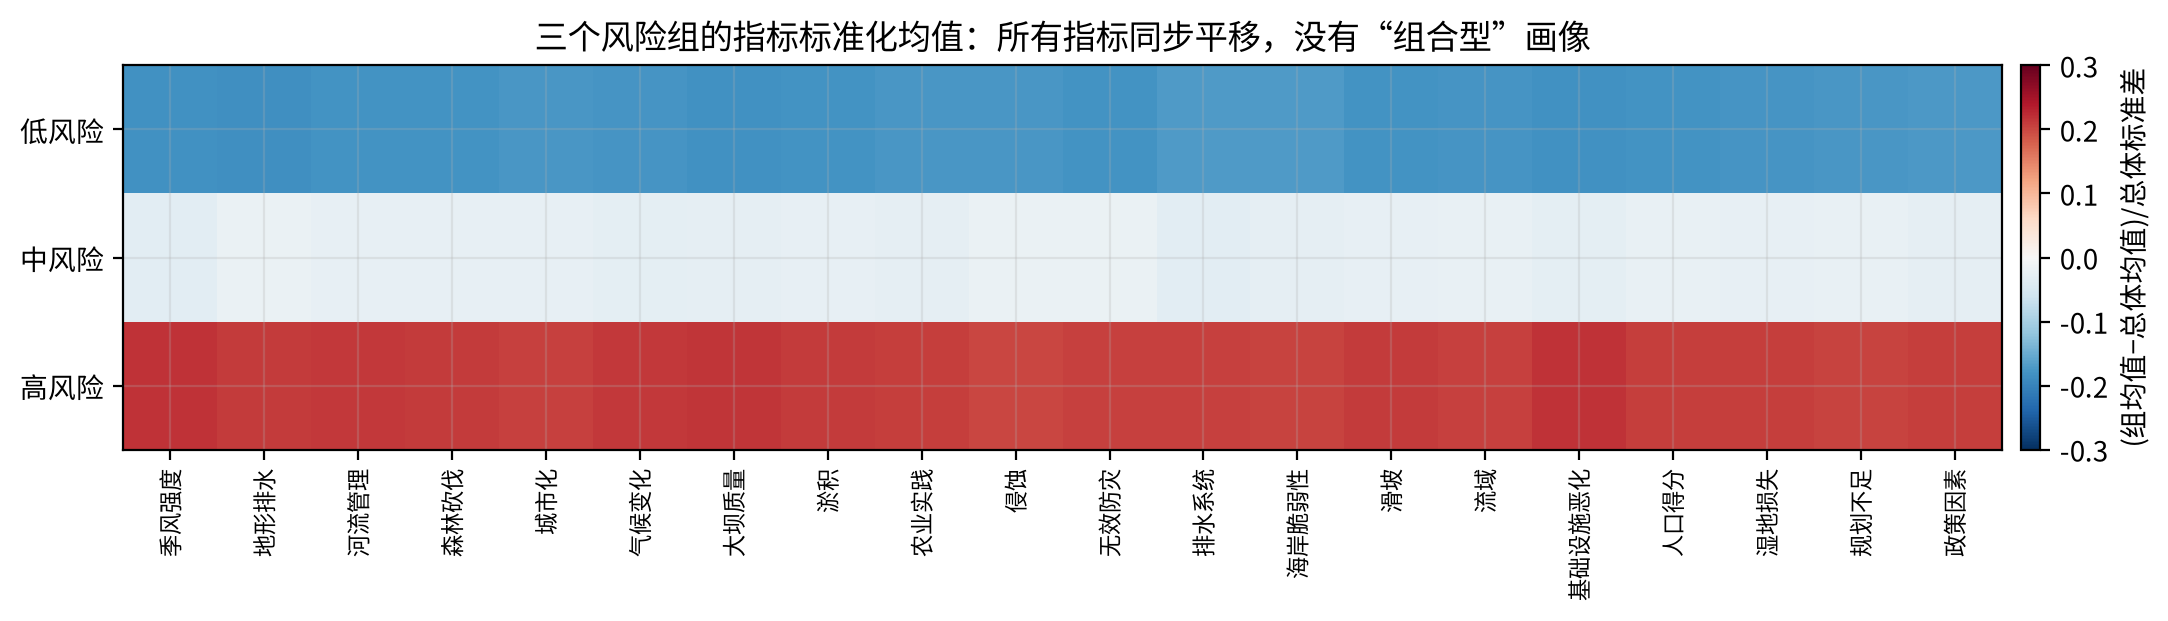
\includegraphics[width=\textwidth]{../figures/fig_p2_profiles.png}
\caption{三个风险组的指标标准化均值：所有指标同步平移}
\label{fig:p2profiles}
\end{figure}

作为对照，直接对 20 维标准化指标做 KMeans（$k=3$），得到的三个簇与风险三分位的调整兰德指数（ARI）仅为 $7.3\times10^{-5}$，三个簇的目标均值都约为 0.504。这说明：\textbf{在特征空间里聚类找不到风险类型，风险只能由总量（或目标）定义}。

\subsection{赋权}
分别用熵权法、CRITIC、PCA 第一主成分和等权计算权重：
\begin{itemize}
  \item 熵权：权重范围 $[0.04887,0.05107]$，最大/最小比 1.045；
  \item CRITIC：权重范围 $[0.04943,0.05045]$，最大/最小比 1.021；
  \item 等权：全部为 0.05；
  \item PCA 第一主成分：仅解释 5.1\% 的方差，权重最大/最小比 112.6，分布极不均匀。
\end{itemize}
熵权与 CRITIC 都接近等权，这与指标的近似可交换性一致。PCA 不适用，因为数据近似各向同性，第一主成分并不是“风险因子”，而是方差较大的任意方向。

\begin{table}[htbp]
\centering
\caption{四种赋权方法的权重分布}
\label{tab:weights}
\small
\begin{tabular}{lrrrr}
\toprule
方法 & 最小 & 最大 & 最大/最小 & 标准差 \\
\midrule
等权 & 0.0500 & 0.0500 & 1.000 & 0.00000 \\
熵权 & 0.0489 & 0.0511 & 1.045 & 0.00051 \\
CRITIC & 0.0494 & 0.0504 & 1.021 & 0.00031 \\
PCA1 & 0.0016 & 0.1776 & 112.576 & 0.04548 \\
\bottomrule
\end{tabular}
\par\vspace{2pt}\footnotesize 理想等权为 1/20=0.05；PCA 因数据近似各向同性而不适用。
\end{table}


\begin{figure}[H]
\centering
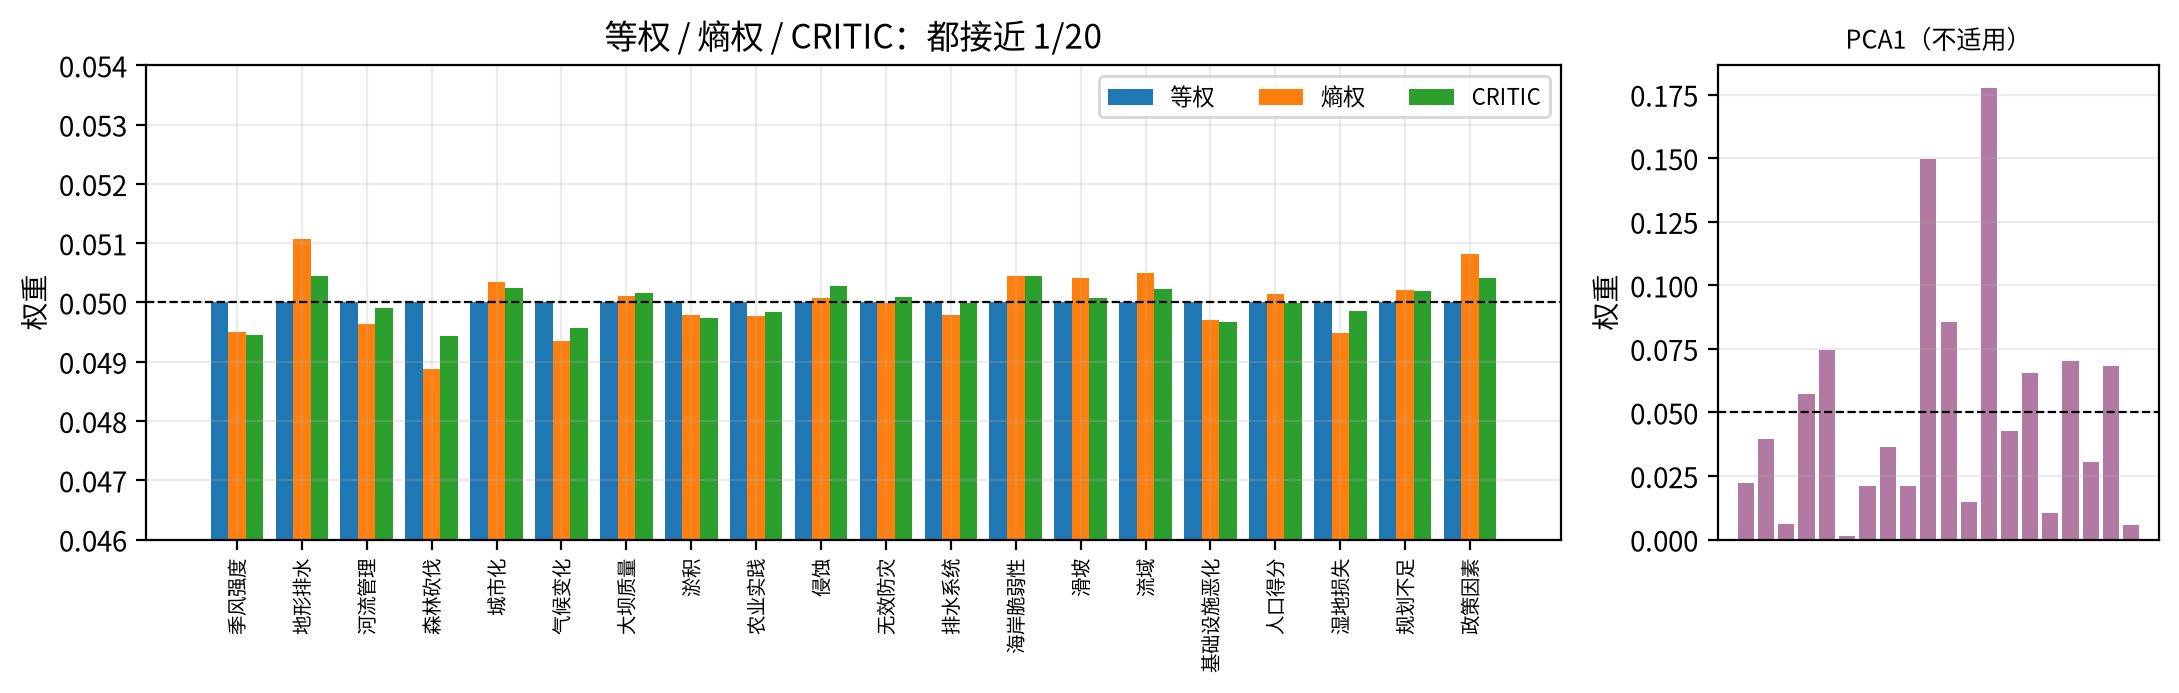
\includegraphics[width=\textwidth]{../figures/fig_p2_weights.png}
\caption{四种赋权结果：熵权、CRITIC、等权都接近 1/20}
\label{fig:p2weights}
\end{figure}

\subsection{TOPSIS 预警模型}
采用 CRITIC 权重，对 20 个指标做向量归一化、加权、取正/负理想解，计算贴近度
\[
C_i=\frac{d_i^-}{d_i^++d_i^-}.
\]
所有指标按“越大风险越高”处理（数据中所有指标与目标正相关）。TOPSIS 得分与目标的 Spearman 为 0.8805，Pearson 为 0.9012，线性校准后 $R^2=0.8122$。按得分三分位划分预警等级，与目标三分位的一致率为 71.5\%；其中高风险识别较准，低/中风险存在一定交叉，这是连续风险分级本身的边界模糊所致。

\begin{table}[htbp]
\centering
\caption{TOPSIS 预警模型与灵敏度}
\label{tab:topsis}
\small
\begin{tabular}{lr}
\toprule
指标 & 数值 \\
\midrule
Spearman（TOPSIS vs 目标） & 0.8805 \\
Pearson（TOPSIS vs 目标） & 0.9012 \\
线性校准后 R² & 0.8122 \\
三级预警一致率 & 71.52\% \\
权重扰动（$\pm10$\%）后 Spearman 均值 & 0.9689 \\
单指标 $\pm20$\% 扰动后 Spearman 范围 & [0.9919,0.9947] \\
KMeans 与三分位的 ARI & 0.0001 \\
风险组 $\eta^2$ 范围 & [0.0236, 0.0271] \\
\bottomrule
\end{tabular}
\end{table}


\begin{figure}[H]
\centering
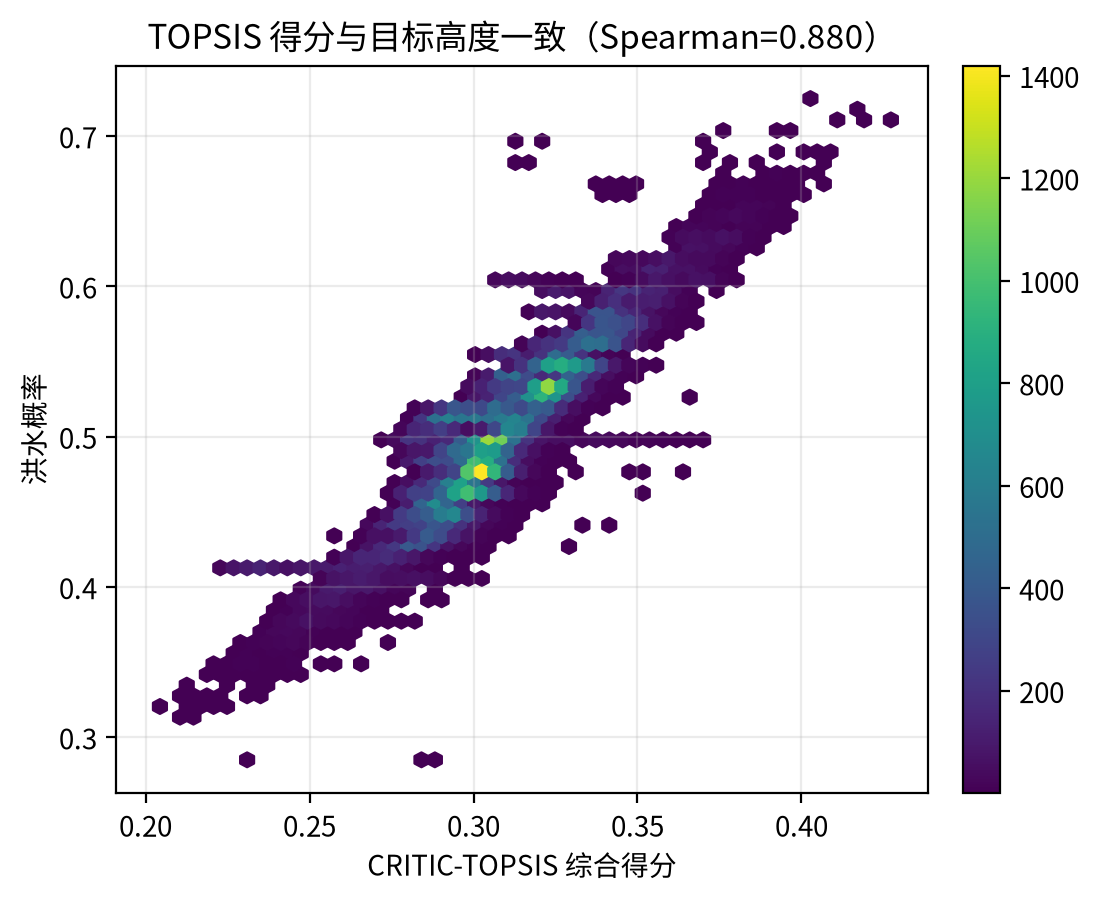
\includegraphics[width=0.62\textwidth]{../figures/fig_p2_topsis.png}
\caption{CRITIC-TOPSIS 得分与洪水概率高度一致}
\label{fig:p2topsis}
\end{figure}

\subsection{灵敏度分析}
\begin{enumerate}
  \item \textbf{权重随机扰动}：围绕 CRITIC 权重生成 300 组 Dirichlet 扰动，权重相对标准差约 9.6\%；TOPSIS 排序与基准的 Spearman 均值为 0.9689，95\% 区间为 $[0.9468,0.9844]$，最小值 0.9371。
  \item \textbf{单指标扰动}：对每个指标单独 $\pm20\%$ 调整权重，排序 Spearman 在 $[0.9919,0.9947]$。
\end{enumerate}
因此，TOPSIS 预警模型对权重不敏感；这也从侧面说明，在等权结构下，权重怎么调都不会产生“某个指标主导”的结果。



\subsection{结论}
问题 2 的预警模型应被理解为一个“综合致灾指数”：
\begin{itemize}
  \item 权重取熵权/CRITIC/等权均可，差异可忽略；
  \item 风险等级由总分决定，分项只用于解释“为什么总分高”；
  \item 高/中/低风险不是三种不同的指标组合，而是同一组合的不同水平；
  \item 实际预警时，建议报告总分、等级与分项贡献，而不是宣称“某指标是关键”。
\end{itemize}

\section{问题 3：预测模型与五指标改进}

\subsection{模型比较}
将训练集按 80/20 划分（838,860 / 209,715），比较六类模型。结果如下：

\begin{table}[htbp]
\centering
\caption{预测模型在 20\% 验证集上的表现}
\label{tab:models}
\small
\begin{tabular}{lrrr}
\toprule
模型 & RMSE & MAE & $R^2$ \\
\midrule
OLS(20指标) & 0.02011 & 0.01582 & 0.8445 \\
Ridge($\alpha=1$) & 0.02011 & 0.01582 & 0.8445 \\
等权指数 & 0.02011 & 0.01582 & 0.8444 \\
HistGB & 0.02116 & 0.01689 & 0.8277 \\
随机森林 & 0.03533 & 0.02879 & 0.5199 \\
均值基线 & 0.05098 & 0.04087 & -0.0000 \\
\bottomrule
\end{tabular}
\end{table}


OLS、Ridge 与等权指数的验证集 RMSE 均为 0.02011，$R^2$ 约 0.8445，已经达到第 \ref{sec:eda} 节估计的噪声下限。HistGB 的 RMSE 为 0.02116，随机森林为 0.03533，均未超过线性模型；均值基线为 0.05098。这说明目标对指标是近似线性的，复杂模型只会增加方差。





\subsection{特征重要性}
标准化系数全部在 0.2259–0.2322 之间，置换重要性的 RMSE 增量在 0.00581–0.00609 之间，差异极小。与问题 1 一致，特征重要性排序不稳定：置换重要性最高的“海岸脆弱性”在 Pearson 相关中排最后，而 Pearson 最高的“基础设施恶化”在置换重要性中排倒数第二。因此不应据此删减指标。

\subsection{五指标穷举}
题目要求讨论“仅用 5 个关键指标”。由于 20 个指标近似可交换，直觉上任意 5 个都应差不多。为验证这一点，本文利用充分统计量穷举全部 $\binom{20}{5}=15504$ 个组合，对每个组合在训练集上拟合、在验证集上评估。

\begin{table}[htbp]
\centering
\caption{仅用 5 个指标的精度损失（穷举 15504 个组合）}
\label{tab:five}
\small
\begin{tabular}{lrrp{0.42\linewidth}}
\toprule
方案 & RMSE & $R^2$ & 指标组合 \\
\midrule
20 指标（OLS/等权） & 0.02011 & 0.8445 & 全部 20 个 \\
最优 5 指标 & 0.04604 & 0.1844 & 季风强度,地形排水,气候变化,大坝质量,基础设施恶化 \\
最差 5 指标 & 0.04651 & 0.1678 & 城市化,侵蚀,排水系统,海岸脆弱性,流域 \\
边际相关 Top5 & 0.04613 & 0.1813 & 基础设施恶化,季风强度,大坝质量,河流管理,人口得分 \\
全部 15504 组合中位数 & 0.04627 & — & — \\
\bottomrule
\end{tabular}
\par\vspace{2pt}\footnotesize 5 指标组合的 RMSE 全部落在 [0.0460, 0.0465]，说明任选 5 个指标的表现几乎相同。
\end{table}


结果非常集中：全部 15504 个组合的验证集 RMSE 都落在 $[0.04604,0.04651]$，最大值与最小值只差 0.00047。最优五指标组合为“季风强度、地形排水、气候变化、大坝质量、基础设施恶化”，$R^2=0.1844$；最差组合为“城市化、侵蚀、排水系统、海岸脆弱性、流域”，$R^2=0.1678$；按边际相关选的 Top5 也仅 $R^2=0.1813$。与 20 指标的 0.8445 相比，五指标损失了约 78\% 的解释力，RMSE 从 0.0201 升至 0.0460，增加约 129\%。

\begin{figure}[H]
\centering
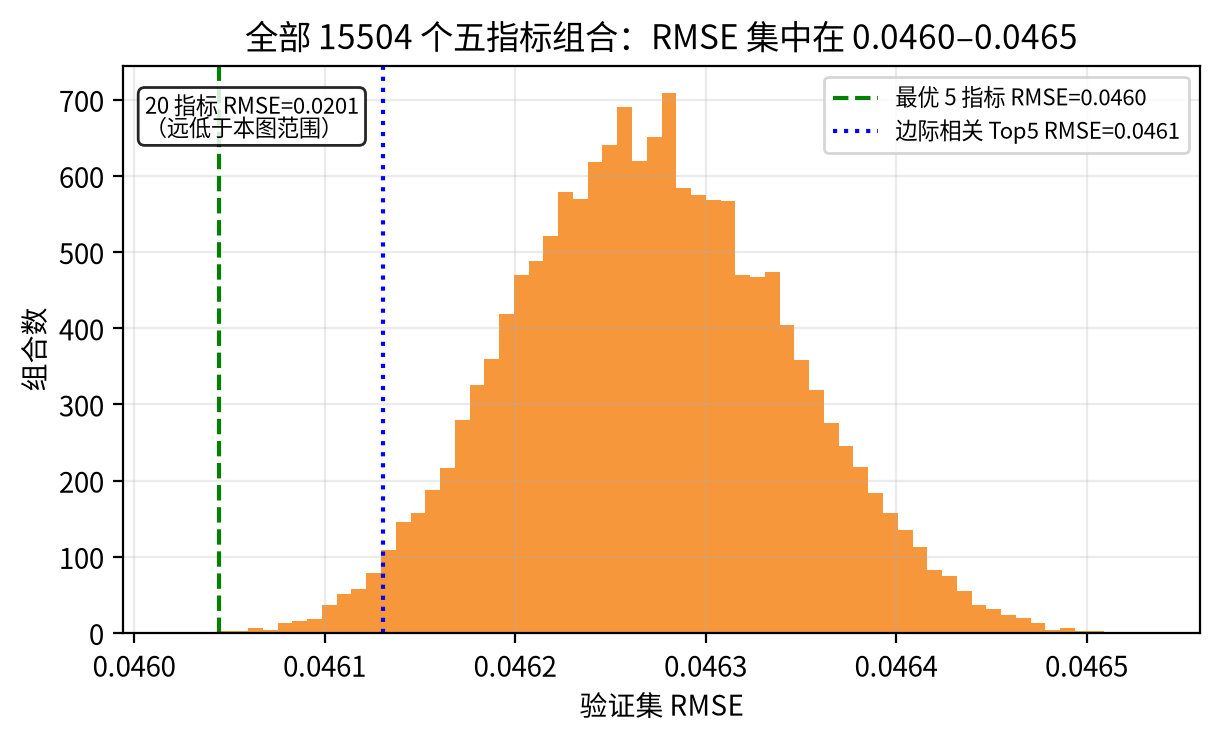
\includegraphics[width=0.7\textwidth]{../figures/fig_p3_five_feature.png}
\caption{全部 15504 个五指标组合的 RMSE 分布}
\label{fig:p3five}
\end{figure}

贪心前向选择的结果也呈平滑下降：加入第 1 个指标 RMSE 约 0.0501，加入第 5 个约 0.0460，加入第 20 个才回到 0.0201。每多一个指标都带来稳定增益，没有“某 5 个就够了”的拐点。

\subsection{学习曲线}
训练样本从 1 万增加到 83.9 万，验证集 RMSE 仅从 0.020129 降到 0.020108。模型只有 20 个参数，1 万样本已足够估计；增加数据不会突破噪声下限。



\subsection{结论}
\begin{enumerate}
  \item 在可部署的单机制模型内，最佳点预测器是 20 指标 OLS（等价于等权指数），验证集 RMSE 0.02011、$R^2$ 0.8445；第 6 节的生成模型也证实 $\mathbb{E}[y|x]=aN+b$，双机制 oracle 只能作为上界、不可部署；
  \item 仅用 5 个指标必然显著降精度，任选 5 个的表现几乎相同；
  \item 若业务上必须只用 5 个，应：选择稳定、可解释、采集成本低的 5 个指标；重新标定系数；明确报告精度损失（RMSE 约 0.046）；不要把 5 指标模型包装成“与 20 指标等效”；
  \item 更合理的低成本方案是“5 个分项 + 1 个综合指数”或“分层抽样监测”，而不是丢弃 15 个指标。
\end{enumerate}

\section{问题 4：测试集预测与分布检验}

\subsection{预测与提交}
用问题 3 的 OLS 模型对 745,305 条测试数据预测，结果统计如下：均值 0.5045、标准差 0.0469、最小值 0.3024、最大值 0.7600、1\% 分位 0.3758、99\% 分位 0.6297。按原附件格式写回 \texttt{submit.csv}：GBK 编码、CRLF 换行、保留末尾两个空列、id 与 \texttt{test.csv} 完全一致、概率保留 6 位小数。

\subsection{分布检验}
对预测概率做正态性检验：
\begin{itemize}
  \item 偏度 0.0824，峰度 0.8411；
  \item KS 检验（对拟合正态）$D=0.0714$，$p<10^{-300}$；
  \item Anderson--Darling 统计量 3540.7，远大于 5\% 临界值 0.752；
  \item Jarque--Bera 统计量 22813.7，$p<10^{-300}$；
  \item Shapiro--Wilk（$n=5000$）$W=0.9850$，$p<10^{-20}$。
\end{itemize}
所有检验都拒绝正态。直方图与核密度显示，预测概率在约 0.47 与 0.54 处有两个主要峰，中间约 0.51 处存在明显低谷。

\begin{table}[htbp]
\centering
\caption{问题 4 预测分布与观测目标的正态性对比}
\label{tab:normality}
\small
\begin{tabular}{lrr}
\toprule
统计量 & 预测概率（信号） & 训练集观测值（信号+噪声） \\
\midrule
均值 & 0.5045 & 0.5045 \\
标准差 & 0.0469 & 0.0510 \\
偏度 & 0.0824 & 0.0481 \\
峰度 & 0.8411 & -0.0390 \\
KS $D$（vs 正态） & 0.0714 & 0.0285 \\
JB 统计量 & 22813.7 & — \\
Shapiro $W$（$n=5000$） & 0.9850 & — \\
\bottomrule
\end{tabular}
\par\vspace{2pt}\footnotesize 预测信号峰度约 0.84，明显偏离正态；观测值叠加噪声后峰度约 $-0.04$。
\end{table}


\begin{figure}[H]
\centering
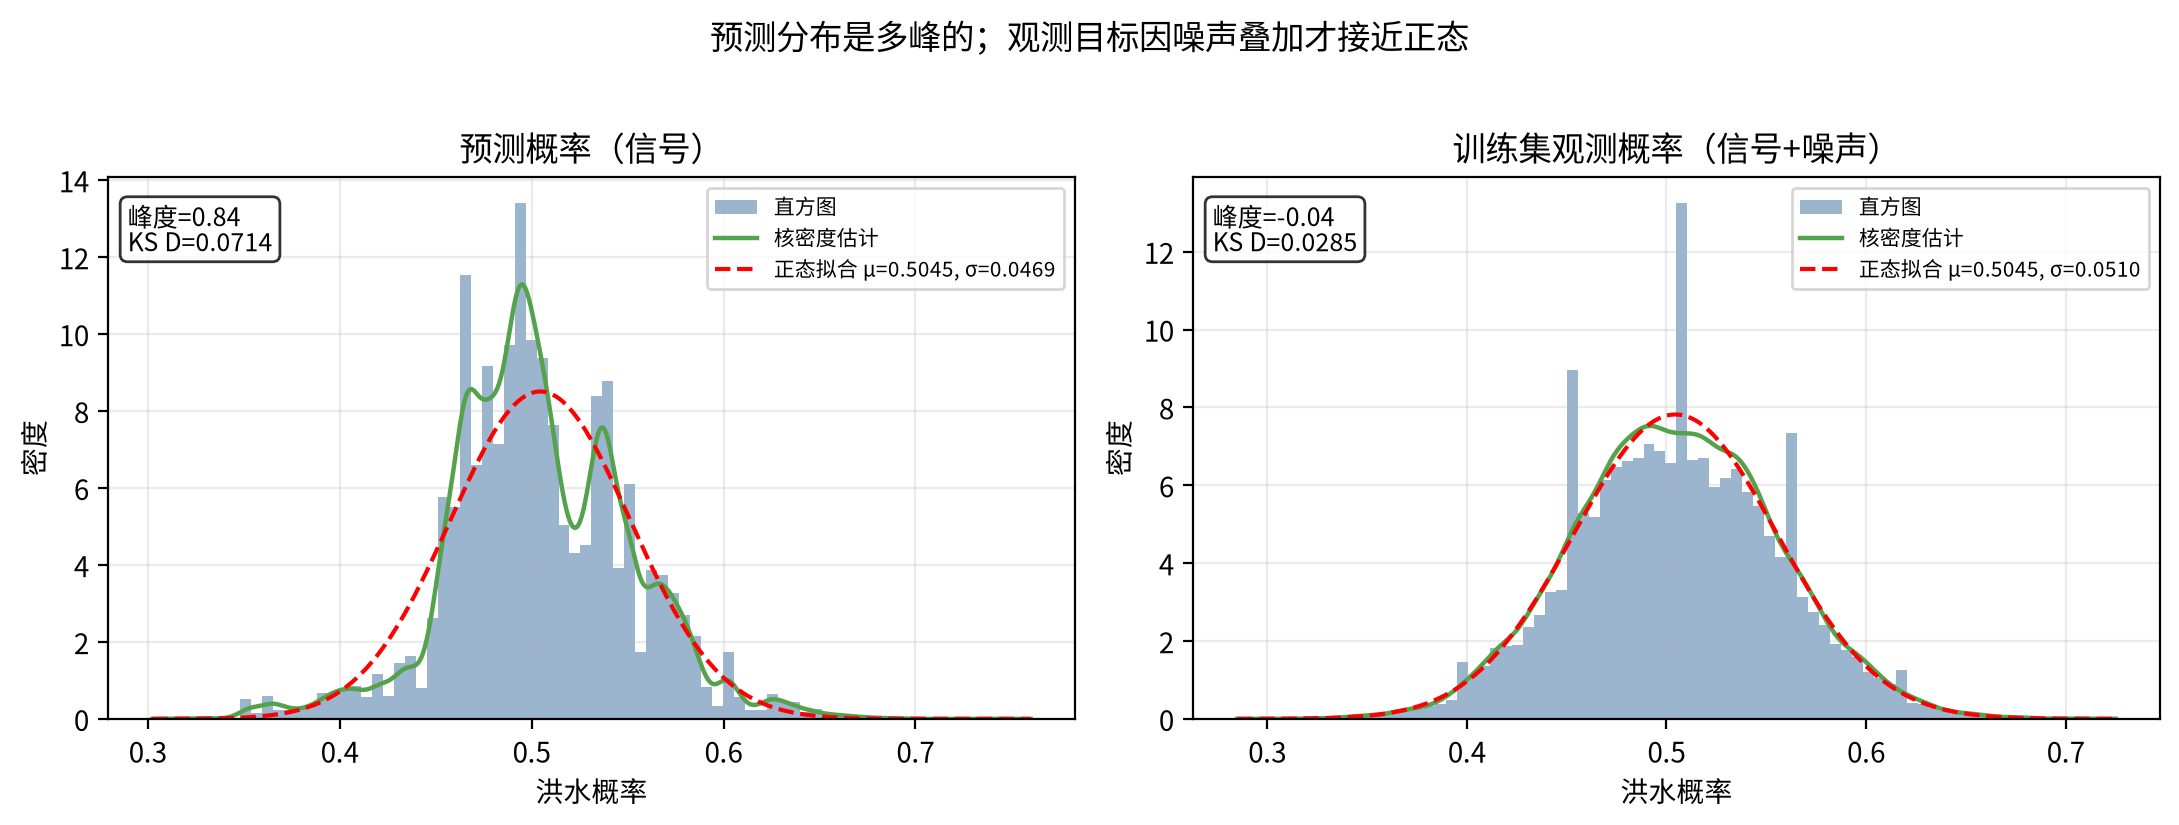
\includegraphics[width=\textwidth]{../figures/fig_p4_hist.png}
\caption{预测信号多峰；观测值因噪声叠加才接近正态}
\label{fig:p4hist}
\end{figure}



\subsection{为什么预测非正态，而观测近似正态？}
由第 \ref{sec:eda} 节，预测信号为 $0.00564676N-0.053355$。$N$ 本身是多峰分布，因此预测信号继承多峰性（峰度 0.841）。训练集观测值 $y$ 等于信号加噪声，噪声标准差 0.0201，相当于约 3.6 个 $N$ 单位，足以把相邻峰之间的低谷部分填平；于是 $y$ 的峰度降到 $-0.039$，KS $D$ 降到 0.0285，在实用意义上接近正态。

因此，对题目“是否服从正态分布”的回答应当是：
\begin{quote}
\textbf{预测信号不服从正态分布，而是多峰分布；训练集观测值因观测噪声叠加而近似正态。}不能仅凭“中心极限定理”就断言预测结果正态，因为 20 个指标并不独立（存在总量守恒的负相关），且行总和本身是多峰混合。
\end{quote}

\section{模型评价与推广}

\subsection{优点}
\begin{enumerate}
  \item \textbf{数据理解深}：不是直接套模型，而是先识别出等权—总量—多项分配结构，后续四问的结论互相印证；
  \item \textbf{证据链完整}：可交换性、负相关、$-1/19$、行总和多峰、目标线性、噪声下限、五指标穷举、预测多峰，形成闭环；
  \item \textbf{机制反演}：不仅拟合预测，还反演出 \(N\) 的 GMM、欠离散多项分配与 Student-\(t\) 噪声，并用后验预测检验复现数据；
  \item \textbf{因果敏感性}：用 DAG、偏相关与干预模拟说明 \(N\) 是混杂变量，避免把边际相关误读为“改某个指标就能降风险”；
  \item \textbf{结论诚实}：明确指出“没有关键指标”“5 指标必然降精度”“预测非正态”，不迎合常规叙事；
  \item \textbf{可复现}：所有数字由 \texttt{run\_all.py} 一键重跑，提交文件格式与原附件一致。
\end{enumerate}

\subsection{局限}
\begin{enumerate}
  \item 数据呈现强生成结构；本文已反演其参数，但真实洪水数据可能包含更复杂的时空/非线性结构，生态效度仍需外部验证；
  \item 风险分级阈值（三分位）与预警等级阈值带有主观性，实际业务应结合成本—损失确定；
  \item 因果部分是 DAG/生成模型假设下的敏感性分析，不是干预实验；潜在机制 \(R\) 不可观测，\(N\to y\) 斜率存在 \(0.0044\)–\(0.0061\) 的异质性，若存在未测混杂，结论需重新审视；
  \item 5 指标的选择只考虑了统计精度，未纳入采集成本、时效性与可操作性。
\end{enumerate}

\subsection{推广}
\begin{itemize}
  \item 对任何“多指标综合评分”数据，先检查行总和、指标相关与可交换性，再决定用加权综合还是多因子模型；
  \item 若指标存在总量约束，应使用成分数据分析（CLR/ILR）或多项分配模型，而不是直接做 PCA/因子分析；
  \item 预警系统可采用“综合指数定级 + 分项诊断 + 不确定性区间”的三层结构；
  \item 对非正态、多峰的预测分布，应报告中位数、分位数与风险区间，而不只报均值。
\end{itemize}

\section*{参考文献}

\noindent\textbf{[1]}\ 2024 年第十四届 APMCM 亚太地区大学生数学建模竞赛（中文赛项）B 题：洪水灾害的数据分析与预测.

\noindent\textbf{[2]}\ Efron B, Tibshirani R J. An Introduction to the Bootstrap. Chapman \& Hall, 1993.

\noindent\textbf{[3]}\ Hastie T, Tibshirani R, Friedman J. The Elements of Statistical Learning. Springer, 2009.

\noindent\textbf{[4]}\ Breiman L. Random Forests. Machine Learning, 2001, 45: 5--32.

\noindent\textbf{[5]}\ Hwang C L, Yoon K. Multiple Attribute Decision Making: Methods and Applications. Springer, 1981.

\noindent\textbf{[6]}\ Diakoulaki D, Mavrotas G, Papayannakis L. Determining objective weights in multiple criteria problems: The CRITIC method. Computers \& Operations Research, 1995, 22(7): 763--770.

\noindent\textbf{[7]}\ Shannon C E. A Mathematical Theory of Communication. Bell System Technical Journal, 1948, 27: 379--423.

\noindent\textbf{[8]}\ Pearl J. Causality: Models, Reasoning, and Inference. 2nd ed. Cambridge University Press, 2009.

\noindent\textbf{[9]}\ Bishop C M. Pattern Recognition and Machine Learning. Springer, 2006.



\section*{附录 A\quad 复现说明}

\begin{verbatim}
cd solution/code
/home/shaun/miniforge3/bin/python run_all.py
\end{verbatim}

运行顺序：\texttt{eda.py} $\to$ \texttt{structure.py} $\to$ \texttt{generative.py} $\to$ \texttt{causal.py} $\to$ \texttt{problem1.py} $\to$ \texttt{problem2.py} $\to$ \texttt{problem3.py} $\to$ \texttt{problem4.py} $\to$ \texttt{make\_tables.py}。全部结果写入 \texttt{results/}，图写入 \texttt{figures/}，提交文件为 \texttt{solution/results/submit.csv}。


\end{document}
